%!TeX root=../pridetop.tex

 \chapter[Chapter \thechapter]{}

\begin{figure}[t!]
\centering
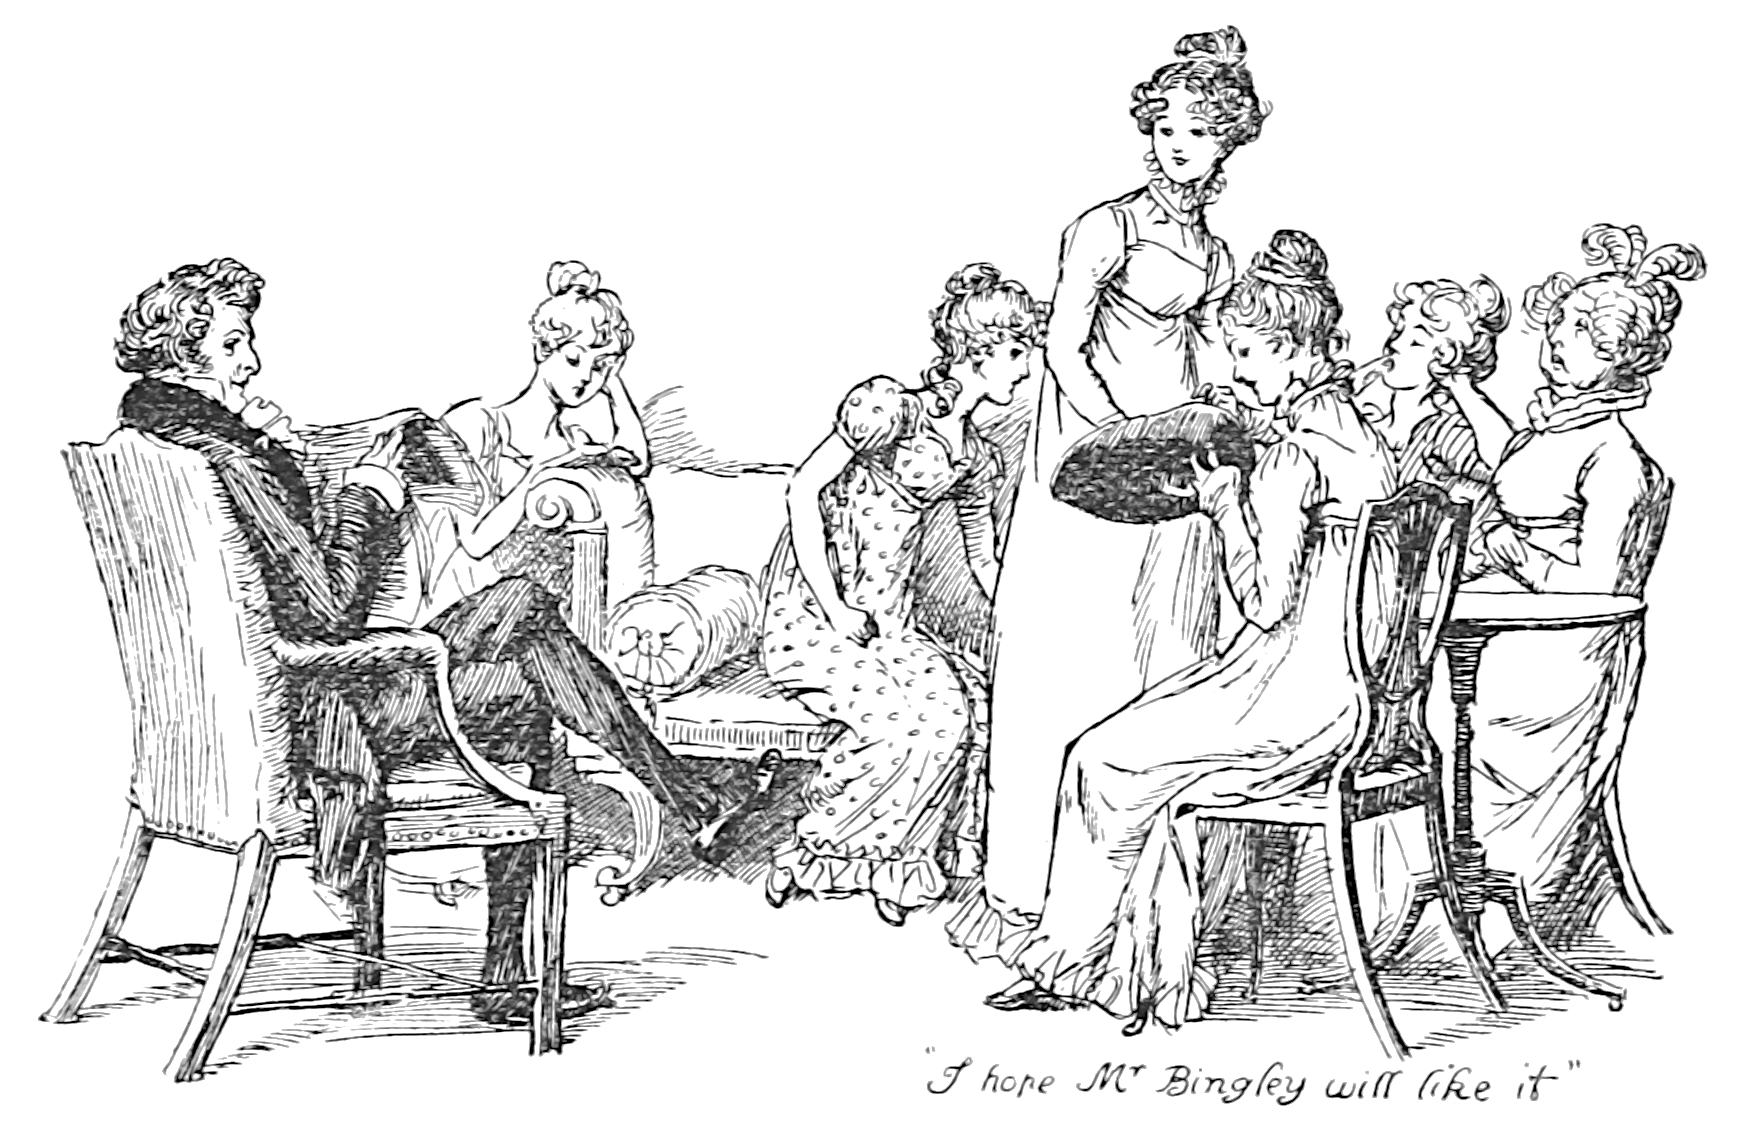
\includegraphics[width=\linewidth]{2top}
\captionlistentry{»I hope Mr Bingley will like it«}
\end{figure}

 \lettrine[lines=6,image=true,findent=5pt]{initials/chap2m}{ Bennet} was among the earliest of those who waited on Mr Bingley. He had always intended to visit him, though to the last always assuring his wife that he should not go; and till the evening after the visit was paid she had no knowledge of it. It was then disclosed in the following manner. Observing his second daughter employed in trimming a hat, he suddenly addressed her with,—

»I hope Mr Bingley will like it, Lizzy.«

»We are not in a way to know \textit{what} Mr Bingley likes,« said her mother, resentfully, »since we are not to visit.«

»But you forget, mamma,« said Elizabeth, »that we shall meet him at the assemblies, and that Mrs Long has promised to introduce him.«

»I do not believe Mrs Long will do any such thing. She has two nieces of her own. She is a selfish, hypocritical woman, and I have no opinion of her.«

»No more have I,« said Mr Bennet; »and I am glad to find that you do not depend on her serving you.«

Mrs Bennet deigned not to make any reply; but, unable to contain herself, began scolding one of her daughters.

»Don't keep coughing so, Kitty, for heaven's sake! Have a little compassion on my nerves. You tear them to pieces.«

»Kitty has no discretion in her coughs,« said her father; »she times them ill.«

»I do not cough for my own amusement,« replied Kitty, fretfully. »When is your next ball to be, Lizzy?«

»To-morrow fortnight.«

»Ay, so it is,« cried her mother, »and Mrs Long does not come back till the day before; so, it will be impossible for her to introduce him, for she will not know him herself.«

»Then, my dear, you may have the advantage of your friend, and introduce Mr Bingley to \textit{her}.«

»Impossible, Mr Bennet, impossible, when I am not acquainted with him myself; how can you be so teasing?«

»I honour your circumspection. A fortnight's acquaintance is certainly very little. One cannot know what a man really is by the end of a fortnight. But if \textit{we} do not venture, somebody else will; and after all, Mrs Long and her nieces must stand their chance; and, therefore, as she will think it an act of kindness, if you decline the office, I will take it on myself.«

The girls stared at their father. Mrs Bennet said only, »Nonsense, nonsense!«

»What can be the meaning of that emphatic exclamation?« cried he. »Do you consider the forms of introduction, and the stress that is laid on them, as nonsense? I cannot quite agree with you \textit{there}. What say you, Mary? For you are a young lady of deep reflection, I know, and read great books, and make extracts.«

Mary wished to say something very sensible, but knew not how.

»While Mary is adjusting her ideas,« he continued, »let us return to Mr Bingley.«

»I am sick of Mr Bingley,« cried his wife.

\begin{figure}[tbh!]
\centering
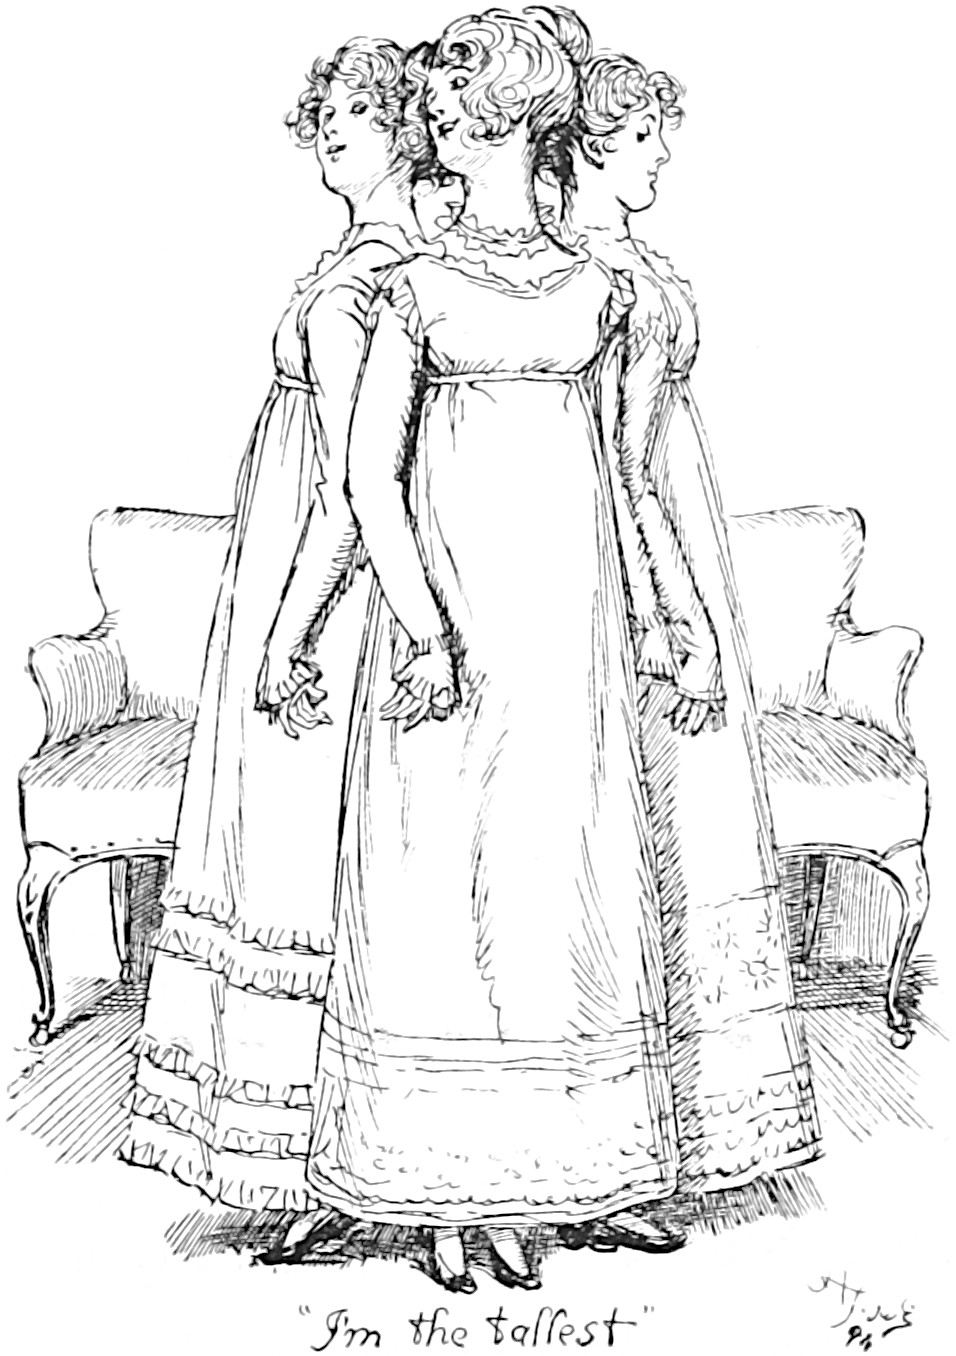
\includegraphics[width=.8\linewidth]{2tallest}
\captionlistentry{»I'm the tallest«}
\end{figure}

»I am sorry to hear \textit{that}; but why did you not tell me so before? If I had known as much this morning, I certainly would not have called on him. It is very unlucky; but as I have actually paid the visit, we cannot escape the acquaintance now.«

The astonishment of the ladies was just what he wished—that of Mrs Bennet perhaps surpassing the rest; though when the first tumult of joy was over, she began to declare that it was what she had expected all the while.

»How good it was in you, my dear Mr Bennet! But I knew I should persuade you at last. I was sure you loved your girls too well to neglect such an acquaintance. Well, how pleased I am! And it is such a good joke, too, that you should have gone this morning, and never said a word about it till now.«

»Now, Kitty, you may cough as much as you choose,« said Mr Bennet; and, as he spoke, he left the room, fatigued with the raptures of his wife.

»What an excellent father you have, girls,« said she, when the door was shut. »I do not know how you will ever make him amends for his kindness; or me either, for that matter. At our time of life, it is not so pleasant, I can tell you, to be making new acquaintances every day; but for your sakes we would do anything. Lydia, my love, though you \textit{are} the youngest, I dare say Mr Bingley will dance with you at the next ball.«

»Oh,« said Lydia, stoutly, »I am not afraid; for though I \textit{am} the youngest, I'm the tallest.«

The rest of the evening was spent in conjecturing how soon he would return Mr Bennet's visit, and determining when they should ask him to dinner.